\documentclass[]{article}
\usepackage{mathtools,amssymb,amsthm,url,cancel,tensor,fancyhdr,graphicx}
\newtheorem{theorem}{Theorem}
\newcommand\numberthis{\addtocounter{equation}{1}\tag{\theequation}}
\fancyhead[L]{}
\fancyhead[C]{
	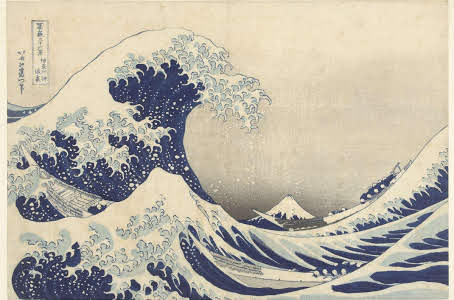
\includegraphics[width=6cm]{kanagawa.jpg}
}

\setlength\headheight{60pt} 

\graphicspath{ {images/} }

\pagestyle{plain}

% Title Page
\title{Introduction into General Relativity\\Assignment 9.1\\Gravitational Waves I}
\author{Simon Crase}


\begin{document}
\maketitle
\thispagestyle{fancy}
\raggedright

\begin{theorem}
	\begin{align*}
	0 =& D_{\mu} T^{\mu}_{\nu} \numberthis\label{eq:continuity} \\
	\equiv & \partial_{\mu} T^{\mu}_{\nu} + \Gamma^{\mu}_{\beta\mu}T^{\beta}_{\nu}-\Gamma^{\beta}_{\nu\mu}T^{\mu}_{\beta} \numberthis\label{eq:covariant-derivative}\\
	\equiv& \frac{1}{\sqrt(|g|)}\partial_{\mu}(T^{\mu}_{\nu}\sqrt{(|g|)}) - \frac{1}{2}(\partial_{\nu}g_{\mu\alpha})T^{\mu\alpha} \numberthis\label{eq:final}
	\end{align*}
\end{theorem}

\begin{proof}
	\begin{align*}
	D_{\alpha} T^{\mu}_{\nu} 
	\equiv & \partial_{\alpha} T^{\mu}_{\nu} + \Gamma^{\mu}_{\beta\alpha}T^{\beta}_{\nu}-\Gamma^{\beta}_{\nu\alpha}T^{\mu}_{\beta} \text{, from \cite[(34)]{akhmedev2016}}\\
	D_{\mu} T^{\mu}_{\nu}
	\equiv & \partial_{\mu} T^{\mu}_{\nu} + \Gamma^{\mu}_{\beta\mu}T^{\beta}_{\nu}-\Gamma^{\beta}_{\nu\mu}T^{\mu}_{\beta}\text{, upon contracting $\mu$ and $\alpha$}
	\end{align*}
	Now (\ref{eq:continuity}) is merely the covariant conservation law, \cite[(80)]{akhmedev2016}, so we can rewrite the foregoing,
	$\partial_{\mu} T^{\mu}_{\nu} + \Gamma^{\mu}_{\beta\mu}T^{\beta}_{\nu}-\Gamma^{\beta}_{\nu\mu}T^{\mu}_{\beta}=0$, which is the same as equation (\ref{eq:covariant-derivative}). We will derive (\ref{eq:final}) by simplifying (\ref{eq:covariant-derivative}), which we repeat for convenience.
	\begin{align*}
	0= & \underbrace{\partial_{\mu} T^{\mu}_{\nu} + \Gamma^{\mu}_{\beta\mu}T^{\beta}_{\nu}}_\text{I}-\underbrace{\Gamma^{\beta}_{\nu\mu}T^{\mu}_{\beta}}_\text{II}\numberthis\label{eq:restated}
	\end{align*}
	We can rewrite the first term in (\ref{eq:restated})
	\begin{align*}
		\frac{1}{\sqrt(|g|)}\partial_{\mu}(T^{\mu}_{\nu}\sqrt{(|g|)}) =&\partial_{\mu}T^{\mu}_{\nu} + T^{\mu}_{\nu}\frac{\partial_{\mu}\sqrt(|g|)}{\sqrt(|g|)} \numberthis\label{eq:term1}
	\end{align*}
	Where we have used a well known result (e.g. \cite[equation (3.11)]{abs1965}), $\Gamma^{\alpha}_{\rho\alpha}=\frac{1}{2|g|}\big(\partial_\rho \, |g|\big)$.
	
	We next expand the second term in (\ref{eq:restated}) and use $g^{\alpha\beta}=g^{\beta\alpha}$ 
	\begin{align*}
	\Gamma^{\beta}_{\nu\mu}T^{\mu}_{\beta} \triangleq& \frac{1}{2} g^{\alpha\beta} \big( \partial_{\nu}g_{\alpha\mu} + \partial_{\mu}g_{\nu\alpha} - \partial_{\alpha}g_{\mu\nu}\big) T^{\mu}_{\beta}\text{, \cite[(46)]{akhmedev2016}}\\
	=&\frac{1}{2} (\partial_{\nu}g_{\alpha\mu})T^{\mu\alpha} + \frac{1}{2}  (\partial_{\mu}g_{\nu\alpha})T^{\mu\alpha} - \frac{1}{2}  (\partial_{\alpha}g_{\mu\nu}) T^{\mu\alpha}\text{, raising index}\\
	=&\frac{1}{2} (\partial_{\nu}g_{\alpha\mu})T^{\mu\alpha} + \frac{1}{2}  (\partial_{\mu}g_{\nu\alpha})T^{\mu\alpha} - \frac{1}{2}  (\partial_{\mu'}g_{\alpha'\nu}) T^{\alpha'\mu'}\text{, relabelling indices } (\mu,\alpha)\rightarrow(\alpha',\mu')\\
	=&\frac{1}{2} (\partial_{\nu}g_{\alpha\mu})T^{\mu\alpha} + \frac{1}{2}  (\partial_{\mu}g_{\nu\alpha})T^{\mu\alpha} - \frac{1}{2}  (\partial_{\mu}g_{\alpha\nu}) T^{\alpha\mu} \text{, dropping primes}\\
	=&\frac{1}{2} (\partial_{\nu}g_{\alpha\mu})T^{\mu\alpha} + \cancel{\frac{1}{2}  (\partial_{\mu}g_{\nu\alpha})T^{\mu\alpha}} - \cancel{\frac{1}{2}  (\partial_{\mu}g_{\nu\alpha}) T^{\mu\alpha}}\text{, symmetry of $g_{\mu\alpha}$ and $T^{\mu\alpha}$}\\
	=&\frac{1}{2} (\partial_{\nu}g_{\alpha\mu})T^{\mu\alpha} \numberthis\label{eq:term2}
	\end{align*}
	Substituting (\ref{eq:term1}) and (\ref{eq:term2}) in (\ref{eq:restated}), we have
	\begin{equation*}
	\frac{1}{\sqrt(|g|)}\partial_{\mu}(T^{\mu}_{\nu}\sqrt{(|g|)}) - \frac{1}{2}(\partial_{\nu}g_{\mu\alpha})T^{\mu\alpha}=0\text{, matching equation (\ref{eq:final})}
	\end{equation*}
\end{proof}

\begin{theorem}
	If we choose a reference system at a point $x_0$ such that $\partial_{\alpha}g_{\mu\nu}(x_0)=0$, but $\partial_{\alpha}\partial_{\beta}g_{\mu\nu}(x_0)\neq0$, then
	\begin{align*}
	R^{\mu\nu}(x_0) = & \frac{1}{2}g^{\mu\alpha}g^{\nu\gamma}g^{\sigma\delta}\big[\partial_{\alpha}\partial_{\delta}g_{\sigma\gamma} + \partial_{\sigma}\partial_{\gamma}g_{\alpha\delta} - \partial_{\alpha}\partial_{\gamma}g_{\sigma\delta} - \partial_{\sigma}\partial_{\delta}g_{\alpha\gamma}\big] \numberthis\label{eq:R} \\
	T^{\mu\nu}(x_0) =& \partial_{\alpha}\bigg\{ \frac{1}{16\pi\kappa}\frac{1}{|g|}\partial_{\beta}\big[|g|(g^{\mu\nu}g^{\alpha\beta}-g^{\mu\alpha}g^{\nu\beta})\big]\bigg\} \numberthis  \label{eq:T} \\
	\equiv& \frac{1}{|g|}\partial_{\alpha}\eta^{\mu\nu\alpha} \text{, where }
	\eta^{\mu\nu\alpha} = \frac{1}{16\pi\kappa} \partial_{\beta} \big[|g|(g^{\mu\nu}g^{\alpha\beta}-g^{\mu\alpha}g^{\nu\beta})\big] \numberthis\label{eq:eta}
	\end{align*}
\end{theorem}

\begin{proof}
	From \cite[(53)]{akhmedev2016}
	\begin{align*}
	R\indices{^{\mu}_{\nu\alpha\beta}}(x_0) =& \partial_{\alpha}\Gamma^{\mu}_{\nu\beta}(x_0) - \partial_{\beta}\Gamma^{\mu}_{\nu\alpha}(x_0) + \underbrace{\Gamma^{\mu}_{\gamma\alpha}(x_0)\Gamma^{\nu}_{\mu\beta}(x_0)-\Gamma^{\mu}_{\gamma\beta}(x_0) \Gamma^{\gamma}_{\nu\alpha}(x_0)}_\text{$=0$, since $\partial_{\alpha}g_{\mu\nu}(x_0)=0$}\\
	=& \partial_{\alpha}\Gamma^{\mu}_{\nu\beta}(x_0) - \partial_{\beta}\Gamma^{\mu}_{\nu\alpha}(x_0) \numberthis\label{eq:rdef}
	\end{align*}
	Hence
	\begin{align*}
	R_{\mu\nu}(x_0) \triangleq&R\indices{^{\alpha}_{\mu\alpha\nu}}(x_0)\\
	R^{\mu\nu}(x_0)=& g^{\mu\rho}(x_0)g^{\nu\sigma}(x_0) R\indices{^{\alpha}_{\rho\alpha\sigma}}(x_0)\\
	=&g^{\mu\rho}(x_0)g^{\nu\sigma}(x_0)\big(\underbrace{\partial_{\alpha}\Gamma^{\alpha}_{\rho\sigma}(x_0)}_\text{First term} -\underbrace{ \partial_{\sigma}\Gamma^{\alpha}_{\rho\alpha}(x_0)}_\text{Second term} \big) \text{, from (\ref{eq:rdef})} \numberthis\label{eq:RR}
	\end{align*}
	Expanding the first term from (\ref{eq:RR})
	\begin{align*}
	\partial_{\alpha}\Gamma^{\alpha}_{\rho\sigma}(x_0) =& \frac{1}{2}\partial_{\alpha}\big[g^{\alpha\beta}\big(\partial_{\sigma}g_{\beta\rho} + \partial_{\rho} g_{\sigma\beta} - \partial_{\beta} g_{\rho\sigma}\big)\big]\\
	 =& \frac{1}{2}\big[ (\partial_{\alpha}g^{\alpha\beta})\big(\underbrace{\partial_{\sigma}g_{\beta\rho} + \partial_{\rho} g_{\sigma\beta} - \partial_{\beta}g_{\rho\sigma}}_\text{$=0$, for $x=x_0$}\big) + g^{\alpha\beta}\partial_{\alpha}\big(\partial_{\sigma}g_{\beta\rho} + \partial_{\rho} g_{\sigma\beta} - \partial_{\beta}g_{\rho\sigma}\big) \big]\\
	 =& \frac{1}{2} g^{\alpha\beta}\big(\partial_{\alpha}\partial_{\sigma}g_{\beta\rho} + \partial_{\alpha}\partial_{\rho} g_{\sigma\beta} - \partial_{\alpha}\partial_{\beta}g_{\rho\sigma}\big) \numberthis\label{eq:D1}
	 \end{align*}
	 Similarly, expanding the second term from (\ref{eq:RR}),
	 \begin{align*} \partial_{\sigma}\Gamma^{\alpha}_{\rho\alpha}(x_0) =& \frac{1}{2}\partial_{\sigma}\big[g^{\alpha\beta}\big(\partial_{\alpha}g_{\beta\rho} + \partial_{\rho}g_{\alpha\beta} - \partial_{\beta}g_{\rho\alpha}\big)\big]\\
	 =& \frac{1}{2}\big[g^{\alpha\beta}\big(\partial_{\sigma}\partial_{\alpha}g_{\beta\rho} + \partial_{\sigma}\partial_{\rho}g_{\alpha\beta} - \partial_{\sigma}\partial_{\beta}g_{\rho\alpha}\big)\big] \numberthis\label{eq:D2}
	\end{align*}
	Substituting (\ref{eq:D1}) and (\ref{eq:D2}) in (\ref{eq:RR}), and using $\partial_{\alpha}\partial_{\sigma}g_{\beta\rho}=\partial_{\sigma}\partial_{\alpha}g_{\beta\rho},$
	\begin{align*}
	R^{\mu\nu}(x_0)=& \frac{1}{2} g^{\mu\rho}(x_0)g^{\nu\sigma}(x_0)g^{\alpha\beta}\big(\cancel{\partial_{\alpha}\partial_{\sigma}g_{\beta\rho}} + \partial_{\alpha}\partial_{\rho} g_{\sigma\beta} - \partial_{\alpha}\partial_{\beta}g_{\rho\sigma} - \cancel{\partial_{\sigma}\partial_{\alpha}g_{\beta\rho}} - \partial_{\sigma}\partial_{\rho}g_{\alpha\beta} + \partial_{\sigma}\partial_{\beta}g_{\rho\alpha}\big)\\
	=& \frac{1}{2} g^{\mu\rho}(x_0)g^{\nu\sigma}(x_0)g^{\alpha\beta}\big( \partial_{\alpha}\partial_{\rho} g_{\sigma\beta} - \partial_{\alpha}\partial_{\beta}g_{\rho\sigma}  - \partial_{\sigma}\partial_{\rho}g_{\alpha\beta} + \partial_{\sigma}\partial_{\beta}g_{\rho\alpha}\big)\\
	&\text{relabelling } \{\rho\rightarrow \alpha \text{, } \sigma\rightarrow\gamma \text{, } \alpha\rightarrow\delta\text{, } \beta\rightarrow\sigma\} \text{ and grouping positive terms together}\\
	=& \frac{1}{2} g^{\mu\alpha}g^{\nu\gamma}g^{\delta\sigma} \big( \partial_{\delta}\partial_{\alpha}g_{\gamma\sigma} + \partial_{\gamma}\partial_{\sigma}g_{\alpha\delta} - \partial_{\delta}\partial_{\sigma}g_{\alpha\gamma} - \partial_{\gamma}\partial_{\alpha}g_{\delta\sigma}\big)\\
	=& \frac{1}{2} g^{\mu\alpha}g^{\nu\gamma}g^{\delta\sigma} \big( \partial_{\alpha}\partial_{\delta}g_{\gamma\sigma} + \partial_{\sigma}\partial_{\gamma}g_{\alpha\delta} - \partial_{\sigma}\partial_{\delta}g_{\alpha\gamma} - \partial_{\alpha}\partial_{\gamma}g_{\delta\sigma}\big) \text{, symmetry of $\partial_{\alpha}\partial_{\delta}$} \\
	=& \frac{1}{2} g^{\mu\alpha}g^{\nu\gamma}g^{\delta\sigma} \big( \partial_{\alpha}\partial_{\delta}g_{\sigma\gamma} + \partial_{\sigma}\partial_{\gamma}g_{\alpha\delta} - \partial_{\sigma}\partial_{\delta}g_{\alpha\gamma} - \partial_{\alpha}\partial_{\gamma}g_{\sigma\delta}\big) \text {, symmetry of $g_{\mu\nu}$}\\
	= & \frac{1}{2}g^{\mu\alpha}g^{\nu\gamma}g^{\sigma\delta}\big[\partial_{\alpha}\partial_{\delta}g_{\sigma\gamma} + \partial_{\sigma}\partial_{\gamma}g_{\alpha\delta} - \partial_{\alpha}\partial_{\gamma}g_{\sigma\delta} - \partial_{\sigma}\partial_{\delta}g_{\alpha\gamma}\big] \text{, on rearranging terms}\\
	\end{align*}
	This matches (\ref{eq:R}).
	
	
	As a first step for proving (\ref{eq:T}), we note that $T^{\mu\nu}=\frac{1}{8\pi\kappa}\big[R^{\mu\nu}-\frac{1}{2}g^{\mu\nu}R\big]$. Furthermore,
	\begin{align*}
	R=&\frac{1}{2}g_{\mu\nu}g^{\mu\alpha}g^{\nu\alpha}g^{\sigma\delta}\big[\partial_{\alpha}\partial_{\delta}g_{\sigma\gamma} + \partial_{\sigma}\partial_{\gamma}g_{\alpha\delta} - \partial_{\alpha}\partial_{\gamma}g_{\sigma\delta} - \partial_{\sigma}\partial_{\delta}g_{\alpha\gamma}\big]\\
	=&\frac{1}{2}\delta^{\alpha}_{\nu}g^{\nu\alpha}g^{\sigma\delta}\big[\partial_{\alpha}\partial_{\delta}g_{\sigma\gamma} + \partial_{\sigma}\partial_{\gamma}g_{\alpha\delta} - \partial_{\alpha}\partial_{\gamma}g_{\sigma\delta} - \partial_{\sigma}\partial_{\delta}g_{\alpha\gamma}\big]\\
	=&\frac{1}{2}g^{\alpha\gamma}g^{\sigma\delta}\big[\partial_{\alpha}\partial_{\delta}g_{\sigma\gamma} + \partial_{\sigma}\partial_{\gamma}g_{\alpha\delta} - \partial_{\alpha}\partial_{\gamma}g_{\sigma\delta} - \partial_{\sigma}\partial_{\delta}g_{\alpha\gamma}\big]
	\end{align*}
	Whence
	\begin{align*}
	T^{\mu\nu}=&\frac{1}{8\pi\kappa}\big[R^{\mu\nu}-\frac{1}{2}g^{\mu\nu}R\big]\\
	=&\frac{1}{8\pi\kappa}\big[ g^{\mu\alpha}g^{\nu\gamma} - \frac{1}{2}g^{\mu\nu}g^{\alpha\gamma}  \big]g^{\sigma\delta}\big[\partial_{\alpha}\partial_{\delta}g_{\sigma\gamma} + \partial_{\sigma}\partial_{\gamma}g_{\alpha\delta} - \partial_{\alpha}\partial_{\gamma}g_{\sigma\delta} - \partial_{\sigma}\partial_{\delta}g_{\alpha\gamma}\big]
	\end{align*}
\end{proof}

\begin{thebibliography}{9}
	
	\bibitem{akhmedev2016}
	Emil T. Akhmedev,
	\emph{Lectures on General Theory of Relativity},
	2016,
	\url{https://arxiv.org/pdf/1601.04996v6.pdf}.
	\bibitem{abs1965}
	Ronald Adler, Maurice Bazin, \& Menahem Schiffer,
	\emph{Introduction to General Relativity},
	McGraw-Hill Book Company, New York,
	1965.
	
	
\end{thebibliography}

\end{document}          
